\documentclass[conference]{IEEEtran}
\usepackage{times}

% numbers option provides compact numerical references in the text.
\usepackage[numbers]{natbib}
\usepackage{multicol}
\usepackage[bookmarks=true]{hyperref}

\usepackage{graphicx} % more modern
%\usepackage{epsfig} % less modern
\usepackage{subfigure}

% For algorithms
\usepackage{algorithm}
\usepackage{algorithmic}
\usepackage{amsmath}
\usepackage{amssymb}
% Include other packages here, before hyperref.
\usepackage{color}
\usepackage{setspace}
\usepackage{wrapfig}
\usepackage{dsfont}

\usepackage[it,small]{caption}


\newcommand{\argmax}{\operatorname{arg\,max}}
\newcommand{\argmin}{\operatorname{arg\,min}}
\newcommand{\todo}[1]{\textcolor{blue}{\textbf{#1}}}
\newtheorem{mydef}{Definition}



\graphicspath{{./images/}}
\usepackage{multirow}
% Some illegal space-saving macros
%  \parskip=5pt
%  \abovedisplayskip 3.0pt plus2pt minus2pt%
% \belowdisplayskip \abovedisplayskip
% \renewcommand{\baselinestretch}{0.97}



\newenvironment{packed_enum}{
\begin{enumerate}
  \setlength{\itemsep}{0pt}
  \setlength{\parskip}{0pt}
  \setlength{\parsep}{0pt}
}
{\end{enumerate}}

\newenvironment{packed_item}{
\begin{itemize}
  \setlength{\itemsep}{0pt}
  \setlength{\parskip}{0pt}
  \setlength{\parsep}{0pt}
}{\end{itemize}}


 \newlength\savedwidth
 \newcommand\whline[1]{\noalign{\global\savedwidth\arrayrulewidth
								\global\arrayrulewidth #1} %
					   \hline
					   \noalign{\global\arrayrulewidth\savedwidth}}
 \renewcommand\multirowsetup{\centering}


\newlength{\sectionReduceTop}
\newlength{\sectionReduceBot}
\newlength{\subsectionReduceTop}
\newlength{\subsectionReduceBot}
\newlength{\abstractReduceTop}
\newlength{\abstractReduceBot}
\newlength{\captionReduceTop}
\newlength{\captionReduceBot}
%\newlength{\nameReduceTop}
\newlength{\subsubsectionReduceTop}
\newlength{\subsubsectionReduceBot}

\newlength{\horSkip}
\newlength{\verSkip}

\newlength{\figureHeight}
\setlength{\figureHeight}{1.7in}

%\newlength{\figureFraction}
\setlength{\horSkip}{-.09in}
\setlength{\verSkip}{-.1in}
%\setlength{\figureFraction}{.195}


%
\setlength{\subsectionReduceTop}{-0.05in}
\setlength{\subsectionReduceBot}{-0.15in}
\setlength{\sectionReduceTop}{-0.07in}
\setlength{\sectionReduceBot}{-0.1in}
\setlength{\subsubsectionReduceTop}{-0.06in}
\setlength{\subsubsectionReduceBot}{-0.05in}
%
%
%\setlength{\figureHeight}{1.5in}
\setlength{\abstractReduceTop}{-0.10in}
\setlength{\abstractReduceBot}{-0.05in}
%
%

%\setlength{\nameReduceTop}{-0.05in}


\setlength{\captionReduceTop}{-0.15in}
\setlength{\captionReduceBot}{-0.15in}



\pdfinfo{
   /Author (Homer Simpson)
   /Title  (Robots: Our new overlords)
   /CreationDate (D:20101201120000)
   /Subject (Robots)
   /Keywords (Robots;Overlords)
}

\usepackage{helvet}
%\renewcommand{\familydefault}{\sfdefault}

\begin{document}


% paper title
\title{Supplementary Material For \\ rCRF: Recursive Belief Estimation over CRFs in RGB-D Activity Videos}

% You will get a Paper-ID when submitting a pdf file to the conference system
%\author{Author Names Omitted for Anonymous Review. Paper-ID 63}
\author{
\authorblockN{Ozan Sener}
\authorblockA{School of Electrical \& Computer Eng. \\ Cornell University}
\and
\authorblockN{Ashutosh Saxena}
\authorblockA{Department of Computer Science \\ Cornell University}
}


\maketitle

\IEEEpeerreviewmaketitle
\section{Resulting Algorithm}
\section{Overview}
\vspace{\subsectionReduceTop}
\label{overview}
\begin{figure}[h!]
  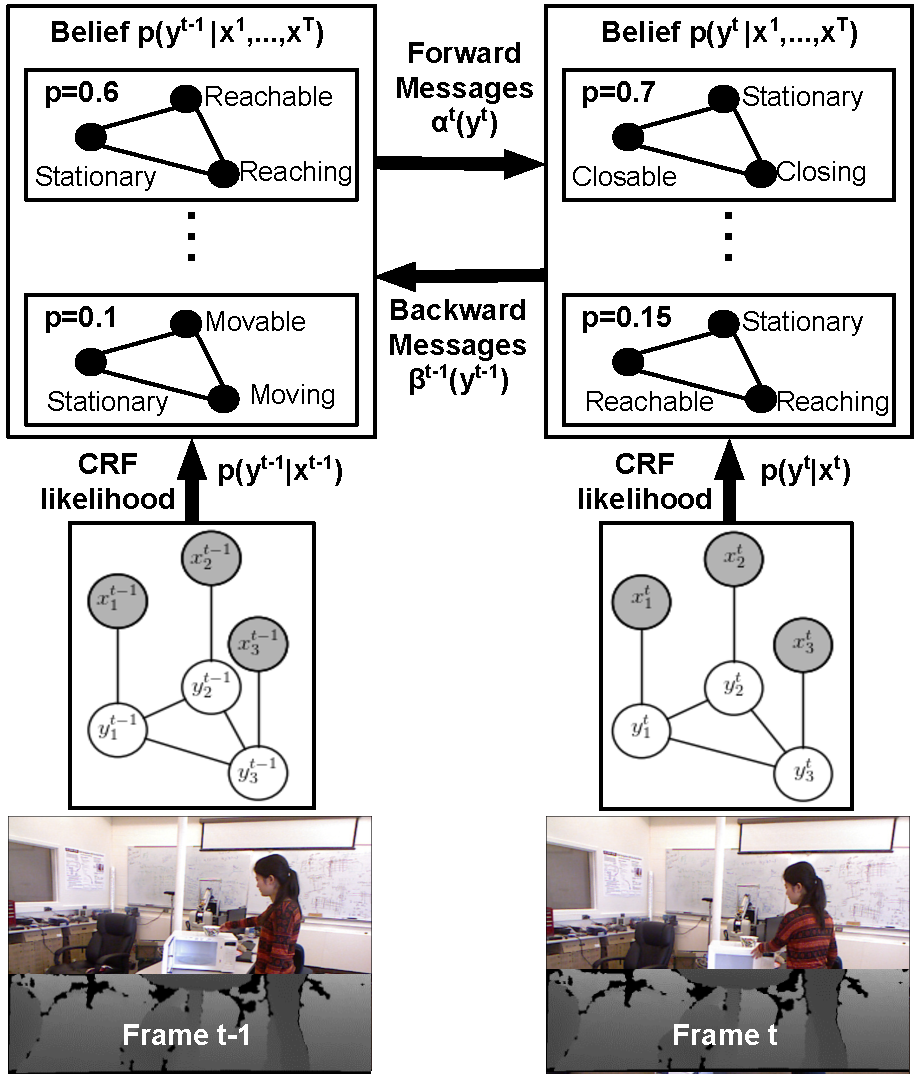
\includegraphics[width=0.49\textwidth]{systemflow}
  \vspace{\captionReduceTop}
  \caption{{\bf Computing the full belief by using rCRF.} Each iteration of the recursive estimation algorithm includes computing forward and backward messages, $\alpha^t(\mathbf{y}^t)$ and $\beta^{t-1}(\mathbf{y}^{t-1})$, by using the current samples and computing the belief $p(\mathbf{y}^t|\mathbf{x}^1,\ldots,\mathbf{x}^T)$ with the computed messages. Then, we re-compute the messages and re-sample the belief until the belief converges. \emph{Here, we only have two objects as  $\mathbf{y}^t=(\mathbf{O}^t_1,\mathbf{O}^t_2,\mathbf{A}^t)$ and $\mathbf{x}^t=(\mathbf{L}^t_1,\mathbf{L}^t_2,\mathbf{H}^t)$ }}
  \vspace{\captionReduceBot}
  \label{system}
\end{figure}
%Toy Example
\end{document}
